\documentclass[12pt]{article}

% PACKAGE IMPORTS (ERT template)
\usepackage{fancyhdr}
\usepackage[utf8]{inputenc}
\usepackage[T1]{fontenc}
\usepackage[english]{babel}
\usepackage{graphicx}
\usepackage{titlesec}
\usepackage{csquotes}
\usepackage{enumitem}
\usepackage{amsfonts}
\usepackage[font=small,skip=0pt]{caption}
\usepackage{subcaption}
\usepackage{hyperref}
\hypersetup{hidelinks}
\usepackage{float}
\usepackage{xcolor}
\usepackage{amsmath,amssymb}
\usepackage{booktabs}
\usepackage{adjustbox}
\usepackage{calc}
\usepackage{colortbl}
\usepackage{array}
\usepackage{etoolbox}
\usepackage{ragged2e}
\usepackage{textcomp, gensymb}
\usepackage{tikz}
\usetikzlibrary{positioning,arrows.meta,shapes.misc}
\usepackage{geometry}
\usepackage{lastpage}
\usepackage[scaled]{helvet}
\usepackage{soul}
\usepackage{eso-pic}
\usepackage[useregional]{datetime2}
\usepackage{longtable}
\usepackage{siunitx}
\sisetup{detect-all}
\usepackage{tabularx}
\usepackage{listings}
\usepackage{needspace}

\graphicspath{{pictures/template/}{figures/}}
\renewcommand\familydefault{\sfdefault}

\definecolor{ertred}{RGB}{226,12,24}
\definecolor{codebg}{RGB}{246,246,244}
\definecolor{codekw}{RGB}{38,92,170}
\definecolor{codecm}{RGB}{110,110,104}
\definecolor{codestr}{RGB}{160,60,20}
\definecolor{notebg}{RGB}{238,243,251}

\lstdefinestyle{ert}{basicstyle=\ttfamily\footnotesize, backgroundcolor=\color{codebg}, frame=single,
  rulecolor=\color{codebg}, framesep=3pt, xleftmargin=4pt, xrightmargin=4pt, columns=fullflexible,
  keepspaces=true, breaklines=true, showstringspaces=false, upquote=true,
  keywordstyle=\color{codekw}\bfseries, commentstyle=\color{codecm}\itshape, stringstyle=\color{codestr},
  aboveskip=6pt, belowskip=6pt}
\lstdefinelanguage{yaml}{morecomment=[l]{\#}, morestring=[b]", sensitive=true}
\lstset{style=ert}
\newcommand{\cmd}[1]{\texttt{#1}}
\newcommand{\key}[1]{\texttt{#1}}
% long identifiers in running text may break after an underscore or a dot
\let\ulorig\_
\renewcommand{\_}{\ulorig\allowbreak}
\newcommand{\dotbreak}{.\allowbreak}
\newcommand{\note}[1]{\par\smallskip\noindent\colorbox{notebg}{\parbox{\dimexpr\textwidth-2\fboxsep}{#1}}\par\smallskip}

\geometry{a4paper, inner=20mm, outer=20mm, top=26mm, bottom=30mm, footskip=10mm, headsep=13mm}
\sodef\an{}{.1em}{0.1em}{0.1em}

\newcommand\BackgroundPic{\put(0,0){\parbox[b][\paperheight]{\paperwidth}{\vfill\centering

\includegraphics[width=\paperwidth,height=\paperheight]{pictures/template/c_title-page.png}\vfill}}}

\begin{document}
\setlength{\emergencystretch}{3em}

\AddToShipoutPicture*{\BackgroundPic}
\ClearShipoutPicture

\let\oldheadrule\headrule
\renewcommand{\headrule}{\color{ertred}\oldheadrule}
\renewcommand{\headrulewidth}{1.5pt}
\renewcommand{\footrule}{\hbox to\headwidth{\color{ertred}\leaders\hrule height \footrulewidth\hfill}}
\renewcommand{\footrulewidth}{1.5pt}
\setlength\headheight{48pt}
\pagestyle{fancy}
\fancyhead[C]{\rule[-2ex]{0pt}{2ex} \bf{ \fontsize{12}{5} \selectfont 2027\_C\_FD\_REPORT-3\_NOSE-CONE-TOOL-USER-GUIDE}}
\lhead{
\includegraphics[height=1.5cm]{pictures/template/ert_logo_small}\vspace{-4mm}}
\rhead{
\includegraphics[height=1.5cm]{pictures/template/c_patch.png}\vspace{-4mm}}
\cfoot{}
\fancyfoot[R]{\bf{\thepage/\pageref{LastPage}}}
\fancyfoot[L]{\rule[-2ex]{0pt}{2ex}\bf{EPFL ROCKET TEAM}}

\begin{titlepage}
\vspace*{-2.40cm}
\noindent\hspace*{-1.2cm}
\parbox{\linewidth}{\bfseries\fontsize{34}{38}\selectfont NOSE-CONE DESIGN\\ TOOL: USER GUIDE\\}
\newline\hspace*{-1.2cm}
\parbox{\linewidth}{\bfseries\fontsize{14}{18}\selectfont Fabio Feig - 315169 \\}
\begin{tikzpicture}[remember picture,overlay]
\node[anchor=south east,inner sep=39mm] at (current page.south east) {\parbox[b][-2.37cm][t]{15cm}{\raggedleft
\fontsize{12}{12} \selectfont \normalfont \textbf{Python package \texttt{nosecone} -- version 1.0}}};
\end{tikzpicture}
\begin{tikzpicture}[remember picture,overlay]
\node[anchor=south east,inner sep=39mm] at (current page.south east) {\parbox[b][-0.8cm][t]{15cm}{\raggedleft
\fontsize{12}{12} \selectfont \normalfont Date: \today}};
\end{tikzpicture}
\begin{tikzpicture}[remember picture,overlay]
\node[anchor=south east,inner sep=39mm] at (current page.south east) {\parbox[b][-1.6cm][t]{15cm}{\raggedleft
\fontsize{12}{12} \selectfont \normalfont Doc ID: 2027\_C\_FD\_REPORT-3\_NOSE-CONE-TOOL-USER-GUIDE}};
\end{tikzpicture}
\end{titlepage}

\pagenumbering{roman}
\tableofcontents
\newpage
\pagenumbering{arabic}
\setcounter{page}{1}

\section*{Quick start}
\addcontentsline{toc}{section}{Quick start}

\noindent\textbf{From zero to the Weisshorn results in four commands} (Windows; see Section~\ref{sec:install}
for macOS/Linux):
\begin{lstlisting}[language=bash]
python -m venv .venv
.venv\Scripts\activate
pip install -r requirements.txt
python -m nosecone run configs/weisshorn.yaml
\end{lstlisting}
\note{Then open \texttt{output/weisshorn/summary.md}: it lists every nose of the study, best first, with its
wave drag, apogee, mass, payload room and static-margin change. Figures are in
\texttt{output/weisshorn/figures/}, CAD files (CSV, STL, STEP) in \texttt{output/weisshorn/cad/}.}

\medskip
\noindent\textbf{To study another rocket}, copy \texttt{configs/example\_new\_rocket.yaml}, change the values of
your vehicle (diameter, length, masses, engine, fins) and the noses you want to compare, and run it with the same
command. You never need to edit the Python code for that: every input is in the YAML file. The parameters
are described in Section~\ref{sec:parameters}, the outputs in Section~\ref{sec:outputs}.

\medskip
\noindent\textbf{How this guide is organised.}
\begin{itemize}[leftmargin=*,itemsep=1pt]
\item Section~\ref{sec:scope}: what the tool computes, with which models, and where these models stop being valid.
\item Section~\ref{sec:install}: installation and requirements.
\item Section~\ref{sec:structure}: the repository and what each module does.
\item Section~\ref{sec:parameters}: the configuration file and the parameters you change.
\item Section~\ref{sec:running}: running a single design and a parameter sweep, with worked examples for our 180~mm rocket.
\item Section~\ref{sec:outputs}: how to read the plots and tables.
\item Section~\ref{sec:extending}: adding a profile family, a plot, a parameter, or changing a model.
\end{itemize}

\section{What the Tool Does, and What It Does Not}
\label{sec:scope}

\subsection{Purpose}

The \texttt{nosecone} package helps to choose the outer shape of the nose cone of a supersonic sounding rocket:
its \emph{profile} (cone, ogive, Von K\'arm\'an, \dots), its \emph{fineness ratio} $L/D$ (length over diameter)
and its \emph{tip radius}. It compares candidates on the quantities a design review asks for (apogee, mass,
payload room, stability, heating, manufacturability) and produces the CAD geometry of the selected design. It was
written for the Weisshorn nose cone (2026\_C\_FD\_REPORT-1\_NOSE\_CONE) and reproduces that report exactly, but
every vehicle-specific number is an input, so the same code serves any ERT rocket.

\subsection{What is computed}

Figure~\ref{fig:chain} shows the chain. Everything starts from a YAML configuration file and a database of
nose wave-drag coefficients computed with the tool's own CFD solver.

\begin{figure}[H]
\centering
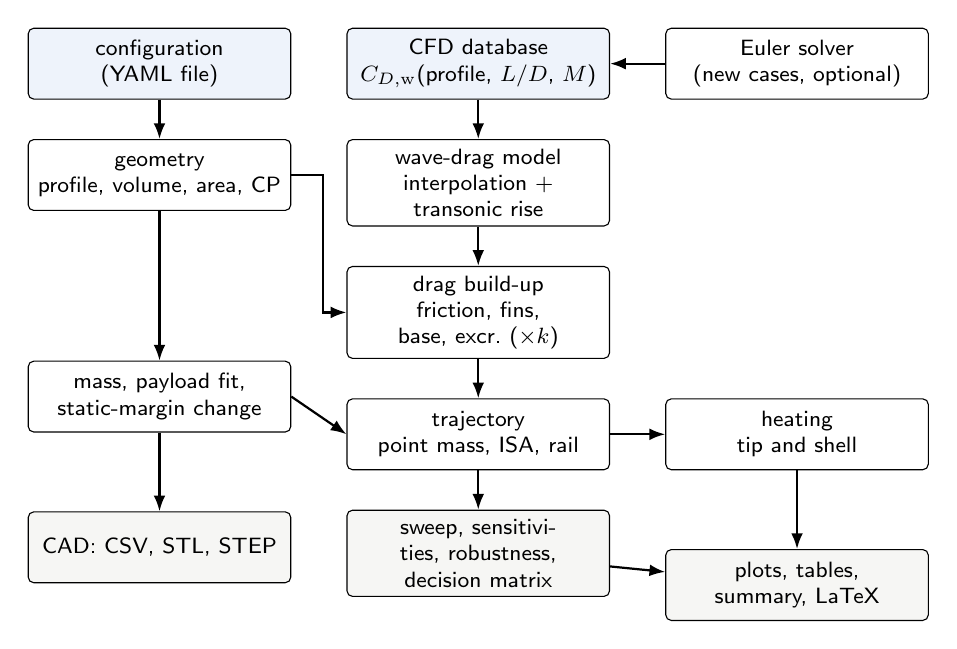
\begin{tikzpicture}[node distance=5mm and 7mm, every node/.style={font=\footnotesize},
  box/.style={draw, rounded corners=2pt, align=center, minimum height=9mm, text width=31mm, fill=white},
  inp/.style={box, fill=notebg}, outp/.style={box, fill=codebg}, arr/.style={-{Latex[length=2mm]}, thick}]
\node[inp] (cfg) {configuration\\(YAML file)};
\node[inp, right=of cfg] (db) {CFD database\\$C_{D,\rm w}$(profile, $L/D$, $M$)};
\node[box, right=of db] (euler) {Euler solver\\(new cases, optional)};
\node[box, below=of db] (wd) {wave-drag model\\interpolation + transonic rise};
\node[box, below=of cfg] (geo) {geometry\\profile, volume, area, CP};
\node[box, below=of wd] (drag) {drag build-up\\friction, fins, base, excr.\ ($\times k$)};
\node[box, below=of drag] (traj) {trajectory\\point mass, ISA, rail};
\node[box, below=of geo, yshift=-14mm] (mass) {mass, payload fit,\\static-margin change};
\node[box, right=of traj] (heat) {heating\\tip and shell};
\node[outp, below=of traj] (res) {sweep, sensitivities, robustness,\\decision matrix};
\node[outp, below=of mass, yshift=-5mm] (cad) {CAD: CSV, STL, STEP};
\node[outp, below=of heat, yshift=-5mm] (out) {plots, tables,\\summary, LaTeX};
\draw[arr] (cfg) -- (geo); \draw[arr] (db) -- (wd); \draw[arr] (euler) -- (db);
\draw[arr] (wd) -- (drag); \draw[arr] (drag) -- (traj); \draw[arr] (geo) -- (mass); \draw[arr] (geo.east) -- ++(4mm,0) |- (drag.west);
\draw[arr] (mass.east) -- (traj.west); \draw[arr] (traj) -- (heat); \draw[arr] (traj) -- (res); \draw[arr] (mass) -- (cad);
\draw[arr] (res) -- (out); \draw[arr] (heat) -- (out);
\end{tikzpicture}
\caption{Computation chain of one run (\texttt{python -m nosecone run}). Shaded blue: inputs; grey: outputs.}
\label{fig:chain}
\end{figure}

For every nose of the sweep (each profile $\times$ each fineness $\times$ each tip radius) the tool computes:
\begin{itemize}[leftmargin=*,itemsep=1pt]
\item \textbf{Geometry}: profile $y(x)$, internal volume, wetted area, angle at the shoulder, tip angle, Barrowman
centre of pressure, length over which the payload fits.
\item \textbf{Wave drag} $C_{D,\rm w}(M)$: the pressure drag of the nose caused by its shock and expansion waves,
read from the CFD database and interpolated.
\item \textbf{Apogee}: a full ascent with the drag of the whole vehicle, the nose length and the nose mass included.
\item \textbf{Mass} of the shell and tip, \textbf{payload fit} and nose-bay length, \textbf{static-margin change}
relative to a baseline nose.
\end{itemize}
For the study as a whole: apogee \textbf{sensitivities} (per kg, per 0.01 of $C_D$), the \textbf{robustness} of
the ranking to the uncertain assumptions, the \textbf{cost of a blunt tip}, the \textbf{temperatures} of the tip
and the shell on a nominal and a hot-day flight, a weighted \textbf{decision matrix}, and the \textbf{CAD files}
of the selected design.

\subsection{Models and their validity}

Table~\ref{tab:models} lists the models. They are deliberately simple and fast (a full study takes minutes), which
is right for comparing shapes, but each has a range outside which its numbers should not be trusted.

\begin{table}[H]
\centering
\caption{Models of the tool and their range of validity.}
\label{tab:models}
\footnotesize
\begin{tabular}{@{}>{\raggedright\arraybackslash}p{2.3cm}>{\raggedright\arraybackslash}p{6.1cm}>{\raggedright\arraybackslash}p{7.6cm}@{}}
\toprule
Quantity & Model & Valid for / limitations \\
\midrule
Wave drag & Axisymmetric Euler CFD (inviscid, zero angle of attack), tabulated at $M = 1.1$--$1.6$ and
$L/D = 3$--$5$ (Weisshorn database) & Supersonic, $1.1 \le M \lesssim 2$; slender noses. Interpolated in $M$ and in
$L/D$ (on $C_{D,\rm w}(L/D)^2$); \emph{held constant} outside the computed range. No viscous effects. \\
Transonic drag & Smooth (cubic) rise from 0 at $M = 0.8$ to the $M = 1.1$ value at $M = 1$ & An assumption, the
weakest part of the chain; checked by the robustness study. Replace by RANS data if available. \\
Rest of the vehicle & Empirical build-up: turbulent flat-plate friction (roughness-limited, compressibility
corrected), fin pressure drag (Ackeret), OpenRocket base drag, ERT-Sim excrescences; one factor $k$ &
Order-of-magnitude accuracy only, hence the calibration of $k$ on a known apogee. Trapezoidal fins, no boat tail,
no protuberances. \\
Trajectory & 2D point mass, rail, constant thrust, linear mass decrease, ISA troposphere, no wind & Apogee
estimates and comparisons. No rotation, no 6-DOF, no wind. The atmosphere is valid below
$\approx\SI{11}{km}$; above that use a better model. \\
Stability & Barrowman (subsonic, linear), nose $C_{N\alpha} = 2$ & \emph{Changes} of static margin between noses;
the absolute margin needs the full vehicle (fins, CG) in RocketPy/OpenRocket. \\
Heating & Fay--Riddell stagnation point; turbulent flat plate with Eckert reference temperature; 1D transient
conduction, adiabatic inner face; lumped metal tip & Conservative peak temperatures for $M \lesssim 3$. No
radiation, no internal convection, no transition, no ablation. \\
Mass & Wetted area $\times$ areal density + tip mass & Scaled from an as-built nose; no coupler, payload or bulkhead. \\
\bottomrule
\end{tabular}
\end{table}

\subsection{What the tool does not do}

\begin{itemize}[leftmargin=*,itemsep=1pt]
\item \textbf{No structural analysis}: no stresses, buckling, flutter or layup design; the mass is an estimate.
\item \textbf{No viscous or transonic CFD}: the solver is inviscid and supersonic. For the final design, run RANS
(e.g.\ Fluent with $k$-$\omega$ SST) at a few Mach numbers.
\item \textbf{No angle of attack}: normal force and centre of pressure come from Barrowman's formulas, not CFD.
\item \textbf{No full-vehicle flight simulation}: use RocketPy with the exported $C_{D,\rm w}(M)$ and geometry.
\item \textbf{No automatic optimisation}: the tool evaluates the noses you list; it does not search for a new shape.
\item \textbf{No new CFD unless asked}: a profile, fineness or tip radius missing from the database is skipped with
a message, unless \key{aerodynamics.compute\_missing} is true (then the Euler solver runs, several minutes per case).
\end{itemize}

\subsection{Reproducibility}

The tool was refactored from the scripts that produced the Weisshorn design report and checked against them:
with \texttt{configs/weisshorn.yaml} it reproduces the report's tables, quoted numbers, CAD files and figures
exactly (Appendix~\ref{app:verification}). \texttt{tests/verify\_reference.py} repeats that check; run it after
any change to the code.

\section{Installation and Requirements}
\label{sec:install}

\subsection{Requirements}

\begin{itemize}[leftmargin=*,itemsep=1pt]
\item \textbf{Python 3.11 or newer} (developed with 3.14) and \texttt{git} to get the repository.
\item The Python packages of \texttt{requirements.txt}: NumPy, SciPy, pandas, Matplotlib, PyYAML and, optionally,
gmsh. The first four are pinned to the versions that produced the Weisshorn report, so that the results are
reproduced bit for bit; newer versions give the same results to about $10^{-12}$.
\item \textbf{Optional: a LaTeX installation} (MiKTeX on Windows, TeX Live on Linux/macOS). With it, the plots use
LaTeX fonts and are identical to the report figures; without it, Matplotlib's built-in renderer is used
automatically and the plots look slightly different but contain the same information.
\item \textbf{Optional: gmsh} (installed by \texttt{requirements.txt}, $\approx$\SI{70}{MB}) for the STEP export.
Without it the STEP file is skipped with a message; the CSV and STL files are always written.
\end{itemize}

\subsection{Installation}

Get the repository (private: ask for access, or download it as a zip from GitHub) and install the packages in a
virtual environment, so that they do not interfere with other Python projects:
\begin{lstlisting}[language=bash]
git clone https://github.com/Landonowins/weisshorn-nose-cone.git
cd weisshorn-nose-cone
python -m venv .venv
.venv\Scripts\activate              # Windows (PowerShell or cmd)
source .venv/bin/activate           # macOS / Linux
pip install -r requirements.txt
\end{lstlisting}
The virtual environment must be activated (the prompt shows \texttt{(.venv)}) in every new terminal before using
the tool. All commands of this guide are run from the repository folder.

\subsection{Checking the installation}

\begin{lstlisting}[language=bash]
python -m nosecone --version                     # prints: nosecone 1.0.0
python -m nosecone validate configs/weisshorn.yaml
python tests/verify_reference.py                 # about 2 minutes; must end with "All outputs match"
\end{lstlisting}

\note{\textbf{Common problems.}
\emph{``No module named nosecone''}: you are not in the repository folder, or the virtual environment is not
active. \emph{LaTeX errors in the plots}: set \key{output.text\_renderer: mathtext} or install the missing
LaTeX packages (MiKTeX installs them on the fly if allowed). \emph{``STEP skipped''}: \texttt{pip install gmsh}.}

\section{Repository Structure}
\label{sec:structure}

\needspace{12\baselineskip}
\subsection{Folders}

\begin{lstlisting}[language={}]
weisshorn-nose-cone/
|-- nosecone/              the Python package (all the code)
|   |-- plotting/          figures (style.py, figures.py)
|-- configs/               weisshorn.yaml + worked examples
|-- data/
|   |-- euler_results.csv  CFD database: wave drag of every case
|   |-- euler_sweep_log.csv   run log of the CFD solver
|   |-- cfd/cp/            wall pressure of every CFD point (.npz)
|   |-- cfd/fields/        flow fields at the design fineness
|-- plugins/               example plugin (Section 7.1)
|-- docs/user_guide/       this guide (LaTeX source and PDF)
|-- report/                the Weisshorn nose-cone design report
|-- tests/                 verify_reference.py + reference outputs
|-- legacy/scripts/        the original scripts (not used)
|-- output/                created by the tool (not in git)
|-- requirements.txt, README.md
\end{lstlisting}

\subsection{Modules}

Each module has one job (Table~\ref{tab:modules}). The functions have docstrings and type hints: in Python,
\texttt{help(nosecone.flight.simulate)} prints the documentation of any function.

\begin{table}[H]
\centering
\caption{Modules of the \texttt{nosecone} package, in the order of the computation chain.}
\label{tab:modules}
\footnotesize
\begin{tabular}{@{}>{\raggedright\arraybackslash}p{2.6cm}>{\raggedright\arraybackslash}p{6.4cm}>{\raggedright\arraybackslash}p{7.0cm}@{}}
\toprule
Module & Job & Main contents \\
\midrule
\texttt{config} & Read, complete and check the YAML file & \texttt{load()}, the dataclasses of every section (parameters with unit, range, default, description), \texttt{describe()} \\
\texttt{constants} & Physical constants and model coefficients (the only fixed numbers) & gas constant, $\gamma$, Sutherland, friction, base-drag, heating coefficients, grid-generator constants \\
\texttt{geometry} & Profiles and their geometric properties & profile families and \texttt{register\_family()}, \texttt{radius()}, blunting, \texttt{volume\_and\_area()}, CP, payload length \\
\texttt{euler} & Axisymmetric Euler CFD solver & \texttt{make\_grid()}, \texttt{Mesh}, \texttt{EulerAxi} (HLLC, MUSCL, local time stepping) \\
\texttt{taylor\_maccoll} & Exact cone flow (solver validation) & \texttt{cone\_cp()} \\
\texttt{cfd} & CFD studies and the database & \texttt{run\_jobs()} (parallel), \texttt{rebuild\_database()}, \texttt{load\_database()} \\
\texttt{aerodynamics} & Wave-drag model from the database & \texttt{WaveDrag} (interpolation in $M$ and $L/D$, transonic rise) \\
\texttt{flight} & Atmosphere, drag build-up, trajectory & \texttt{Atmosphere}, \texttt{DragModel}, \texttt{simulate()}, \texttt{calibrate()} \\
\texttt{stability} & Barrowman stability, nose mass & \texttt{fin\_cna\_xcp()}, \texttt{static\_margin\_shift()}, \texttt{nose\_mass()} \\
\texttt{heating} & Tip and shell temperatures & \texttt{h\_stagnation()}, \texttt{h\_turbulent()}, \texttt{wall\_response()}, \texttt{tip\_insert()} \\
\texttt{design} & The study: sweep and derived results & \texttt{Study}: \texttt{sweep()}, \texttt{sensitivities()}, \texttt{robustness()}, \texttt{bluntness()}, \texttt{heating()}, \texttt{trade\_matrix()}, \texttt{catalogue()} \\
\texttt{export} & CAD and meshing files & profile CSV, \texttt{write\_stl()}, \texttt{write\_step()} (gmsh), \texttt{stl\_check()} \\
\texttt{plotting} & All figures & \texttt{figures.PLOTS} (one function per plot), \texttt{PLOT\_DEFAULTS}, \texttt{style} \\
\texttt{reporting} & Tables and summaries & \texttt{summary\_markdown()}, LaTeX tables and macros \\
\texttt{pipeline} & Runs everything in order & \texttt{run()} \\
\texttt{cli} & Command line & \texttt{python -m nosecone <command>} \\
\texttt{plugins}, \texttt{docs} & Plugin loading; documentation helpers & \texttt{load\_plugins()}; parameter tables of this guide \\
\bottomrule
\end{tabular}
\end{table}

\subsection{Using the package from Python}

The command line covers normal use, but every step is also a function. For example, in a Jupyter notebook:
\begin{lstlisting}[language=Python]
from nosecone import config, pipeline
cfg = config.load("configs/weisshorn.yaml")
cfg.nose.fineness = [4.0, 4.25, 4.5]          # change anything before running
res = pipeline.run(cfg, plots=["trade"])
res["trade"].sort_values("apogee")            # pandas DataFrame of the sweep
st = res["study"]                             # the Study object (wave drag, vehicles, ...)
st.wave_drag("vonkarman", 4.5)(1.3)           # C_D,w of a nose at M = 1.3
\end{lstlisting}

\section{The Configuration File}
\label{sec:parameters}

\subsection{How the file works}

A study is described by one YAML file (\texttt{configs/weisshorn.yaml} is the complete, commented example). YAML
is a plain-text format: \emph{sections} contain \emph{parameters} written \texttt{name: value}, indented by two
spaces; lists are written \texttt{[a, b, c]}; everything after \texttt{\#} is a comment.
\begin{lstlisting}[language=yaml]
vehicle:
  diameter: 0.180        # m
  mass_wet: 75.0         # kg
nose:
  profiles: [ogive, power050, vonkarman]
  fineness: [4.0, 4.5, 5.0]
\end{lstlisting}

\begin{itemize}[leftmargin=*,itemsep=1pt]
\item \textbf{Only what differs from the default is needed.} Every parameter has a default
(Section~\ref{sec:paramtables}); a file with only a \texttt{vehicle} section is valid.
\item \textbf{Units are SI} (m, kg, s, N, K) unless the table says otherwise (\textdegree, \textdegree C).
Write lengths in metres: \texttt{diameter: 0.180}, not \texttt{180}.
\item \textbf{Relative paths} (database, output folder, CFD folders, plugins) are relative to the file that contains them.
\item \textbf{Inheritance}: a file that starts with \texttt{base: weisshorn.yaml} takes every value of that file
and overrides only what it lists (both worked examples of Section~\ref{sec:running} do this). Sections are merged
parameter by parameter; a list given in the new file replaces the inherited list.
\item \textbf{Checking}: \texttt{python -m nosecone validate my.yaml} reads the file and stops at the first problem
with a precise message, e.g.\ \texttt{unknown parameter 'nose.profils' (did you mean 'profiles'?)} or
\texttt{'launch.rail\_elevation' = 95.0 is outside the valid range (0, 90]}. Add \texttt{-{}-show} to print every
value the run will use (defaults included). The same file is saved next to the results as
\texttt{config\_used.yaml}.
\item \textbf{Plugins}: \key{project.plugins} lists Python files imported before the run; they can add profile
families (Section~\ref{sec:newfamily}).
\end{itemize}

\subsection{All parameters}
\label{sec:paramtables}

The tables below are generated from the code (\texttt{python -m nosecone describe-config -{}-latex}), so they always
match the installed version. ``Valid'' gives the accepted range or values; parameters marked $^\ast$ are advanced
numerical settings that normally stay at their default. Parameters whose default is ``see text'' are structured
values, described in Section~\ref{sec:structured}.

\subsection*{\texttt{project}: Project}
\addcontentsline{toc}{subsection}{\texttt{project}: Project}
{\footnotesize
\begin{longtable}{@{}>{\raggedright\arraybackslash}p{3.3cm}>{\raggedright\arraybackslash}p{2.6cm}>{\raggedright\arraybackslash}p{1.3cm}>{\raggedright\arraybackslash}p{1.9cm}>{\raggedright\arraybackslash}p{6.1cm}@{}}
\toprule Parameter & Default & Unit & Valid & Meaning \\ \midrule \endhead \bottomrule \endfoot
\texttt{name} & \texttt{Weisshorn} & -- & -- & Vehicle or study name, used in plot titles and file names \\
\texttt{output\_dir} & \texttt{output} & path & -- & Folder for all outputs (created if missing) \\
\texttt{plugins} & [\,] & path & -- & Python files imported before the run, e.g. new profile families (see the user guide) \\
\end{longtable}\addtocounter{table}{-1}}

\subsection*{\texttt{vehicle}: Vehicle}
\addcontentsline{toc}{subsection}{\texttt{vehicle}: Vehicle}
{\footnotesize
\begin{longtable}{@{}>{\raggedright\arraybackslash}p{3.3cm}>{\raggedright\arraybackslash}p{2.6cm}>{\raggedright\arraybackslash}p{1.3cm}>{\raggedright\arraybackslash}p{1.9cm}>{\raggedright\arraybackslash}p{6.1cm}@{}}
\toprule Parameter & Default & Unit & Valid & Meaning \\ \midrule \endhead \bottomrule \endfoot
\texttt{diameter} & 0.18 & m & > 0 & External (body) diameter D; the nose base diameter \\
\texttt{length} & 5.4 & m & > 0 & Total vehicle length including the reference nose \\
\texttt{reference\_nose\_length} & 0.72 & m & > 0 & Nose length included in `length`; the body is length - reference\_nose\_length \\
\texttt{mass\_wet} & 75 & kg & > 0 & Lift-off mass \\
\texttt{mass\_dry} & 45 & kg & > 0 & Burn-out mass used by mass\_model 'lvo' \\
\texttt{surface\_roughness} & 2e-05 & m & >= 0 & Equivalent sand roughness of the skin (painted CFRP \~{} 20 um) \\
\texttt{nozzle\_exit\_diameter} & 0.075 & m & >= 0 & Nozzle exit diameter; removed from the base area while burning \\
\end{longtable}\addtocounter{table}{-1}}

\subsection*{\texttt{engine}: Engine}
\addcontentsline{toc}{subsection}{\texttt{engine}: Engine}
{\footnotesize
\begin{longtable}{@{}>{\raggedright\arraybackslash}p{3.3cm}>{\raggedright\arraybackslash}p{2.6cm}>{\raggedright\arraybackslash}p{1.3cm}>{\raggedright\arraybackslash}p{1.9cm}>{\raggedright\arraybackslash}p{6.1cm}@{}}
\toprule Parameter & Default & Unit & Valid & Meaning \\ \midrule \endhead \bottomrule \endfoot
\texttt{thrust} & 4500 & N & > 0 & Thrust (constant over the burn) \\
\texttt{burn\_time} & 9.1 & s & > 0 & Burn duration \\
\texttt{total\_impulse} & 40960 & N s & > 0 & Total impulse (sets the propellant mass for mass\_model 'isp') \\
\texttt{specific\_impulse} & 200 & s & > 0 & Specific impulse (propellant mass = I\_t / (I\_sp g0)) \\
\end{longtable}\addtocounter{table}{-1}}

\subsection*{\texttt{fins}: Fins}
\addcontentsline{toc}{subsection}{\texttt{fins}: Fins}
{\footnotesize
\begin{longtable}{@{}>{\raggedright\arraybackslash}p{3.3cm}>{\raggedright\arraybackslash}p{2.6cm}>{\raggedright\arraybackslash}p{1.3cm}>{\raggedright\arraybackslash}p{1.9cm}>{\raggedright\arraybackslash}p{6.1cm}@{}}
\toprule Parameter & Default & Unit & Valid & Meaning \\ \midrule \endhead \bottomrule \endfoot
\texttt{count} & 4 & -- & [1, 8] & Number of fins \\
\texttt{root\_chord} & 0.3 & m & > 0 & Root chord \\
\texttt{tip\_chord} & 0.12 & m & >= 0 & Tip chord \\
\texttt{span} & 0.16 & m & > 0 & Semi-span (root to tip) \\
\texttt{sweep} & 0.18 & m & >= 0 & Leading-edge sweep length (root LE to tip LE, axial) \\
\texttt{thickness} & 0.005 & m & > 0 & Fin thickness \\
\texttt{edge\_fraction} & 0.15 & -- & (0, 0.5] & Length of each LE/TE wedge of the hexagonal section, as a fraction of the mean chord \\
\end{longtable}\addtocounter{table}{-1}}

\subsection*{\texttt{launch}: Launch}
\addcontentsline{toc}{subsection}{\texttt{launch}: Launch}
{\footnotesize
\begin{longtable}{@{}>{\raggedright\arraybackslash}p{3.3cm}>{\raggedright\arraybackslash}p{2.6cm}>{\raggedright\arraybackslash}p{1.3cm}>{\raggedright\arraybackslash}p{1.9cm}>{\raggedright\arraybackslash}p{6.1cm}@{}}
\toprule Parameter & Default & Unit & Valid & Meaning \\ \midrule \endhead \bottomrule \endfoot
\texttt{rail\_length} & 12 & m & > 0 & Launch rail length \\
\texttt{rail\_elevation} & 84 & \textdegree & (0, 90] & Rail elevation above the horizontal \\
\texttt{site\_altitude} & 0 & m & [-500, 5000] & Launch site altitude above sea level \\
\end{longtable}\addtocounter{table}{-1}}

\subsection*{\texttt{atmosphere}: Atmosphere}
\addcontentsline{toc}{subsection}{\texttt{atmosphere}: Atmosphere}
{\footnotesize
\begin{longtable}{@{}>{\raggedright\arraybackslash}p{3.3cm}>{\raggedright\arraybackslash}p{2.6cm}>{\raggedright\arraybackslash}p{1.3cm}>{\raggedright\arraybackslash}p{1.9cm}>{\raggedright\arraybackslash}p{6.1cm}@{}}
\toprule Parameter & Default & Unit & Valid & Meaning \\ \midrule \endhead \bottomrule \endfoot
\texttt{model} & \texttt{isa\_troposphere} & -- & isa\_troposphere & Atmosphere model \\
\texttt{ground\_temperature} & 288.15 & K & [200, 340] & Temperature at the launch site (288.15 K = ISA) \\
\texttt{ground\_pressure} & 101325 & Pa & > 0 & Pressure at the reference altitude of the model \\
\texttt{lapse\_rate} & 0.0065 & K/m & > 0 & Temperature lapse rate in the troposphere \\
\texttt{tropopause\_temperature} & 216.65 & K & > 0 & Temperature floor (tropopause / lower stratosphere) \\
\end{longtable}\addtocounter{table}{-1}}

\subsection*{\texttt{flight}: Flight model}
\addcontentsline{toc}{subsection}{\texttt{flight}: Flight model}
{\footnotesize
\begin{longtable}{@{}>{\raggedright\arraybackslash}p{3.3cm}>{\raggedright\arraybackslash}p{2.6cm}>{\raggedright\arraybackslash}p{1.3cm}>{\raggedright\arraybackslash}p{1.9cm}>{\raggedright\arraybackslash}p{6.1cm}@{}}
\toprule Parameter & Default & Unit & Valid & Meaning \\ \midrule \endhead \bottomrule \endfoot
\texttt{mass\_model} & \texttt{isp} & -- & isp, lvo & Nominal mass model: 'isp' (propellant = I\_t/(I\_sp g0)) or 'lvo' (wet -> dry) \\
\texttt{calibrate} & \texttt{true} & -- & -- & Scale the non-nose drag by a factor k so that the baseline reaches target\_apogee \\
\texttt{target\_apogee} & 9000 & m & > 0 & Apogee the baseline nose must reach when calibrate is true \\
\texttt{drag\_factor} & 1 & -- & > 0 & Factor k on the non-nose drag when calibrate is false \\
\texttt{calibration\_bracket}\,$^\ast$ & \texttt{[0.3, 1.5]} & -- & -- & Search interval for k \\
\texttt{calibration\_tolerance}\,$^\ast$ & 0.0001 & -- & > 0 & Absolute tolerance on k \\
\texttt{t\_max}\,$^\ast$ & 120 & s & > 0 & Integration time limit (apogee normally ends the integration earlier) \\
\texttt{max\_step}\,$^\ast$ & 0.02 & s & > 0 & Maximum ODE time step \\
\texttt{rtol}\,$^\ast$ & 1e-08 & -- & > 0 & ODE relative tolerance \\
\texttt{atol}\,$^\ast$ & 1e-08 & -- & > 0 & ODE absolute tolerance \\
\texttt{output\_step}\,$^\ast$ & 0.05 & s & > 0 & Output sampling of the trade-study trajectories (sets M\_max) \\
\texttt{detail\_output\_step}\,$^\ast$ & 0.02 & s & > 0 & Output sampling of the trajectories used for heating and plots \\
\texttt{envelope\_mass\_model} & \texttt{lvo} & -- & isp, lvo & Mass model of the hot-day envelope trajectory \\
\texttt{envelope\_ground\_temperature} & 303.15 & K & [200, 340] & Ground temperature of the hot-day envelope \\
\texttt{mass\_sensitivity\_step}\,$^\ast$ & 1 & kg & > 0 & Mass step for the apogee sensitivity dz/dm \\
\texttt{cd\_sensitivity\_step}\,$^\ast$ & 0.01 & -- & > 0 & C\_D step for the apogee sensitivity dz/dC\_D \\
\end{longtable}\addtocounter{table}{-1}}

\subsection*{\texttt{nose}: Nose: design space and selected design}
\addcontentsline{toc}{subsection}{\texttt{nose}: Nose: design space and selected design}
{\footnotesize
\begin{longtable}{@{}>{\raggedright\arraybackslash}p{3.3cm}>{\raggedright\arraybackslash}p{2.6cm}>{\raggedright\arraybackslash}p{1.3cm}>{\raggedright\arraybackslash}p{1.9cm}>{\raggedright\arraybackslash}p{6.1cm}@{}}
\toprule Parameter & Default & Unit & Valid & Meaning \\ \midrule \endhead \bottomrule \endfoot
\texttt{profiles} & see text & -- & -- & Profiles compared in the sweep (built-in names or keys of custom\_profiles) \\
\texttt{fineness} & \texttt{[3, 3.5, 4, 4.5, 5]} & -- & -- & Fineness ratios L/D compared in the sweep \\
\texttt{baseline\_profile} & \texttt{vonkarman} & -- & -- & Reference nose for apogee and static-margin changes \\
\texttt{baseline\_fineness} & 4 & -- & > 0 & Fineness of the reference nose \\
\texttt{baseline\_label} & \texttt{baseline} & -- & -- & How the reference length is called in table captions (e.g. 'LVS length') \\
\texttt{design\_profile} & \texttt{vonkarman} & -- & -- & Selected profile (CAD export, heating, final drawing) \\
\texttt{design\_fineness} & 4.5 & -- & > 0 & Selected fineness L/D \\
\texttt{design\_tip\_radius\_ratio} & 0.05 & -- & [0, 0.5] & Selected spherical tip radius r\_n / R (0 = sharp) \\
\texttt{tip\_radius\_ratios} & \texttt{[0]} & -- & -- & Tip radii r\_n / R compared in the sweep (needs CFD data for each) \\
\texttt{shoulder\_length} & 0.06 & m & >= 0 & Cylindrical shoulder behind the curved part (coupler bond) \\
\texttt{custom\_profiles} & \{\,\} & -- & -- & Extra profiles: name -> \{family: ..., <parameter>: value, label: ...\} \\
\end{longtable}\addtocounter{table}{-1}}

\subsection*{\texttt{aerodynamics}: Aerodynamics (wave-drag model)}
\addcontentsline{toc}{subsection}{\texttt{aerodynamics}: Aerodynamics (wave-drag model)}
{\footnotesize
\begin{longtable}{@{}>{\raggedright\arraybackslash}p{3.3cm}>{\raggedright\arraybackslash}p{2.6cm}>{\raggedright\arraybackslash}p{1.3cm}>{\raggedright\arraybackslash}p{1.9cm}>{\raggedright\arraybackslash}p{6.1cm}@{}}
\toprule Parameter & Default & Unit & Valid & Meaning \\ \midrule \endhead \bottomrule \endfoot
\texttt{database} & \texttt{data/euler\_results.csv} & path & -- & CSV of Euler wave-drag results (non-dimensional, reusable for any diameter) \\
\texttt{user\_database} & (empty) & path & -- & Optional second CSV for cases computed with compute\_missing (empty: they are added to `database`) \\
\texttt{studies} & \texttt{[main, f45]} & -- & -- & Database studies used for the wave-drag model \\
\texttt{grid} & \texttt{medium} & -- & coarse, medium, fine & Grid level of the database rows used \\
\texttt{min\_fineness}\,$^\ast$ & 0 & -- & >= 0 & Database rows below this fineness are ignored \\
\texttt{max\_fineness}\,$^\ast$ & 5 & -- & > 0 & Database rows above this fineness are ignored \\
\texttt{machs} & \texttt{[1.1, 1.2, 1.4, 1.6]} & -- & -- & Supersonic Mach numbers at which the wave drag is tabulated \\
\texttt{transonic\_onset} & 0.8 & -- & [0.5, 1] & Mach number where the nose wave drag starts to rise \\
\texttt{transonic\_full} & 1 & -- & [0.8, 1.2] & Mach number where the rise reaches the value at transonic\_match \\
\texttt{transonic\_match} & 1.1 & -- & [1, 1.5] & Lowest Euler Mach number; the model is flat between transonic\_full and this \\
\texttt{compute\_missing} & \texttt{false} & -- & -- & Run the Euler solver for profiles / fineness / tip radii missing from the database \\
\texttt{missing\_machs} & \texttt{[1.6, 1.4, 1.2, 1.1]} & -- & -- & Mach sequence for cases computed on demand (highest first) \\
\end{longtable}\addtocounter{table}{-1}}

\subsection*{\texttt{payload}: Payload}
\addcontentsline{toc}{subsection}{\texttt{payload}: Payload}
{\footnotesize
\begin{longtable}{@{}>{\raggedright\arraybackslash}p{3.3cm}>{\raggedright\arraybackslash}p{2.6cm}>{\raggedright\arraybackslash}p{1.3cm}>{\raggedright\arraybackslash}p{1.9cm}>{\raggedright\arraybackslash}p{6.1cm}@{}}
\toprule Parameter & Default & Unit & Valid & Meaning \\ \midrule \endhead \bottomrule \endfoot
\texttt{enabled} & \texttt{true} & -- & -- & Evaluate the payload fit and nose-bay length \\
\texttt{name} & \texttt{3U} & -- & -- & Payload name used in labels \\
\texttt{length} & 0.3405 & m & > 0 & Payload length \\
\texttt{width} & 0.1 & m & > 0 & Payload width (square section), used in drawings \\
\texttt{required\_radius} & 0.077 & m & > 0 & Outer nose radius needed to house the payload section (half-diagonal + clearance + guide + shell) \\
\texttt{axial\_clearance} & 0.01 & m & >= 0 & Axial margin for the payload bulkhead \\
\end{longtable}\addtocounter{table}{-1}}

\subsection*{\texttt{structure}: Structure (mass model)}
\addcontentsline{toc}{subsection}{\texttt{structure}: Structure (mass model)}
{\footnotesize
\begin{longtable}{@{}>{\raggedright\arraybackslash}p{3.3cm}>{\raggedright\arraybackslash}p{2.6cm}>{\raggedright\arraybackslash}p{1.3cm}>{\raggedright\arraybackslash}p{1.9cm}>{\raggedright\arraybackslash}p{6.1cm}@{}}
\toprule Parameter & Default & Unit & Valid & Meaning \\ \midrule \endhead \bottomrule \endfoot
\texttt{shell\_areal\_density} & 0.98 & kg/m\textsuperscript{2} & > 0 & Shell mass per wetted area (Firehorn as-built: 0.98) \\
\texttt{tip\_mass} & 0.06 & kg & >= 0 & Machined tip insert mass (same for all profiles) \\
\texttt{shell\_cg\_fraction}\,$^\ast$ & 0.35 & -- & [0, 1] & Shell centre of gravity ahead of the shoulder, as a fraction of L \\
\end{longtable}\addtocounter{table}{-1}}

\subsection*{\texttt{heating}: Heating}
\addcontentsline{toc}{subsection}{\texttt{heating}: Heating}
{\footnotesize
\begin{longtable}{@{}>{\raggedright\arraybackslash}p{3.3cm}>{\raggedright\arraybackslash}p{2.6cm}>{\raggedright\arraybackslash}p{1.3cm}>{\raggedright\arraybackslash}p{1.9cm}>{\raggedright\arraybackslash}p{6.1cm}@{}}
\toprule Parameter & Default & Unit & Valid & Meaning \\ \midrule \endhead \bottomrule \endfoot
\texttt{enabled} & \texttt{true} & -- & -- & Run the heating analysis \\
\texttt{trajectory\_from} & \texttt{design} & -- & design, baseline & Nose used to compute the heating trajectories \\
\texttt{materials} & see text & -- & -- & Material properties: name -> \{label, short (optional), conductivity [W/(m K)], density [kg/m\^{}3], specific\_heat [J/(kg K)]\} \\
\texttt{shell\_material} & \texttt{CFRP} & -- & -- & Shell material (key of materials) \\
\texttt{shell\_thickness} & 0.0012 & m & > 0 & Shell thickness \\
\texttt{shell\_stations} & \texttt{[0.05 m, 0.5 L, 1.0 L]} & -- & -- & Shell stations: 'x m' from the tip or 'f L' as a fraction of L \\
\texttt{tip\_material} & \texttt{Al6082} & -- & -- & Tip insert material (lumped model) \\
\texttt{tip\_length} & 0.08 & m & > 0 & Axial length of the tip insert from the apex \\
\texttt{printed\_tip\_material} & \texttt{PETCF} & -- & -- & Material of the comparison printed tip (1D wall at the stagnation point) \\
\texttt{printed\_tip\_thickness} & 0.004 & m & > 0 & Wall thickness of the printed tip \\
\texttt{wall\_nodes}\,$^\ast$ & 40 & -- & [5, 400] & Nodes through the wall thickness \\
\texttt{bond\_limit} & 120 & \textdegree C & -- & Adhesive temperature limit drawn on the shell plot \\
\texttt{bond\_label} & \texttt{DP490 bond limit} & -- & -- & Label of the adhesive limit \\
\texttt{printed\_tip\_hdt} & \texttt{[70, 80]} & \textdegree C & -- & Heat-deflection temperature range of the printed tip polymer \\
\end{longtable}\addtocounter{table}{-1}}

\subsection*{\texttt{bluntness}: Tip bluntness}
\addcontentsline{toc}{subsection}{\texttt{bluntness}: Tip bluntness}
{\footnotesize
\begin{longtable}{@{}>{\raggedright\arraybackslash}p{3.3cm}>{\raggedright\arraybackslash}p{2.6cm}>{\raggedright\arraybackslash}p{1.3cm}>{\raggedright\arraybackslash}p{1.9cm}>{\raggedright\arraybackslash}p{6.1cm}@{}}
\toprule Parameter & Default & Unit & Valid & Meaning \\ \midrule \endhead \bottomrule \endfoot
\texttt{enabled} & \texttt{true} & -- & -- & Evaluate the tip-bluntness study \\
\texttt{study} & \texttt{blunt} & -- & -- & Database study with blunted noses \\
\texttt{profile} & \texttt{vonkarman} & -- & -- & Profile of the bluntness study \\
\texttt{fineness} & 4 & -- & > 0 & Fineness of the bluntness study \\
\texttt{report\_ratios} & \texttt{[0.05, 0.1]} & -- & -- & Tip radii r\_n/R whose drag and apogee cost are reported \\
\texttt{report\_mach} & 1.4 & -- & [1, 5] & Mach number at which the drag cost of the tip is reported \\
\texttt{radius\_range} & \texttt{[0.002, 0.02]} & m & -- & Tip radius range of the heat-transfer curve \\
\end{longtable}\addtocounter{table}{-1}}

\subsection*{\texttt{robustness}: Robustness}
\addcontentsline{toc}{subsection}{\texttt{robustness}: Robustness}
{\footnotesize
\begin{longtable}{@{}>{\raggedright\arraybackslash}p{3.3cm}>{\raggedright\arraybackslash}p{2.6cm}>{\raggedright\arraybackslash}p{1.3cm}>{\raggedright\arraybackslash}p{1.9cm}>{\raggedright\arraybackslash}p{6.1cm}@{}}
\toprule Parameter & Default & Unit & Valid & Meaning \\ \midrule \endhead \bottomrule \endfoot
\texttt{enabled} & \texttt{true} & -- & -- & Run the robustness study \\
\texttt{fineness} & 4.5 & -- & > 0 & Fineness at which all profiles are compared \\
\texttt{reference\_profile} & \texttt{vonkarman} & -- & -- & Apogees are shown relative to this profile \\
\texttt{band} & 30 & m & >= 0 & Half-width of the 'equivalent' band in the plot \\
\texttt{scenarios} & see text & -- & -- & Scenarios: name + any of transonic\_onset, transonic\_factor, drag\_factor\_scale, mass\_model, ground\_temperature \\
\end{longtable}\addtocounter{table}{-1}}

\subsection*{\texttt{trade\_matrix}: Decision matrix}
\addcontentsline{toc}{subsection}{\texttt{trade\_matrix}: Decision matrix}
{\footnotesize
\begin{longtable}{@{}>{\raggedright\arraybackslash}p{3.3cm}>{\raggedright\arraybackslash}p{2.6cm}>{\raggedright\arraybackslash}p{1.3cm}>{\raggedright\arraybackslash}p{1.9cm}>{\raggedright\arraybackslash}p{6.1cm}@{}}
\toprule Parameter & Default & Unit & Valid & Meaning \\ \midrule \endhead \bottomrule \endfoot
\texttt{enabled} & \texttt{true} & -- & -- & Build the weighted trade matrix \\
\texttt{fineness} & 4.5 & -- & > 0 & Fineness at which the matrix is built \\
\texttt{weights} & see text & -- & -- & Criterion weights (should add up to 1) \\
\texttt{manufacture} & see text & -- & -- & Judgement score per profile (1-5) \\
\texttt{heritage} & see text & -- & -- & Judgement score per profile (1-5) \\
\end{longtable}\addtocounter{table}{-1}}

\subsection*{\texttt{validation}: CFD validation plots}
\addcontentsline{toc}{subsection}{\texttt{validation}: CFD validation plots}
{\footnotesize
\begin{longtable}{@{}>{\raggedright\arraybackslash}p{3.3cm}>{\raggedright\arraybackslash}p{2.6cm}>{\raggedright\arraybackslash}p{1.3cm}>{\raggedright\arraybackslash}p{1.9cm}>{\raggedright\arraybackslash}p{6.1cm}@{}}
\toprule Parameter & Default & Unit & Valid & Meaning \\ \midrule \endhead \bottomrule \endfoot
\texttt{cone\_study} & \texttt{cones} & -- & -- & Database study of sharp cones (compared with Taylor-Maccoll) \\
\texttt{cone\_main\_fineness} & 4 & -- & > 0 & Cone of the main study added to the validation plot \\
\texttt{grid\_study} & \texttt{grid} & -- & -- & Database study of the grid-convergence runs \\
\texttt{grid\_profile} & \texttt{vonkarman} & -- & -- & Profile of the grid study \\
\texttt{grid\_fineness} & 4 & -- & > 0 & Fineness of the grid study \\
\texttt{grid\_machs} & \texttt{[1.4, 1.2]} & -- & -- & Mach numbers of the grid study \\
\end{longtable}\addtocounter{table}{-1}}

\subsection*{\texttt{cfd}: CFD solver and studies}
\addcontentsline{toc}{subsection}{\texttt{cfd}: CFD solver and studies}
{\footnotesize
\begin{longtable}{@{}>{\raggedright\arraybackslash}p{3.3cm}>{\raggedright\arraybackslash}p{2.6cm}>{\raggedright\arraybackslash}p{1.3cm}>{\raggedright\arraybackslash}p{1.9cm}>{\raggedright\arraybackslash}p{6.1cm}@{}}
\toprule Parameter & Default & Unit & Valid & Meaning \\ \midrule \endhead \bottomrule \endfoot
\texttt{cp\_dir} & \texttt{data/cfd/cp} & path & -- & Folder of the wall-pressure files (one .npz per case) \\
\texttt{fields\_dir} & \texttt{data/cfd/fields} & path & -- & Folder of the saved flow fields \\
\texttt{log} & \texttt{data/euler\_sweep\_log.csv} & path & -- & Run log appended by the solver \\
\texttt{workers} & 4 & -- & [1, 64] & Parallel processes \\
\texttt{cfl} & 0.85 & -- & [0.05, 1] & CFL number of the local time stepping \\
\texttt{fallback\_cfl}\,$^\ast$ & 0.5 & -- & [0.05, 1] & CFL of the restart from free stream if a run diverges \\
\texttt{max\_iter} & 6000 & -- & >= 100 & Iteration limit per Mach number \\
\texttt{fine\_iter\_factor}\,$^\ast$ & 2 & -- & [1, 10] & Iteration-limit multiplier on the fine grid \\
\texttt{tolerance} & 2e-05 & -- & > 0 & Convergence: relative change of C\_D,w over `check` iterations \\
\texttt{check}\,$^\ast$ & 250 & -- & >= 10 & Iterations between convergence checks \\
\texttt{first\_order\_iters}\,$^\ast$ & 300 & -- & >= 0 & First-order iterations at the start of the first Mach number \\
\texttt{grids} & see text & -- & -- & Grid levels: name -> [cells along nose, cells along cylinder, cells normal, first-cell height / R] \\
\texttt{cylinder\_length}\,$^\ast$ & 5 & R & > 0 & Cylinder behind the nose in the CFD domain \\
\texttt{upstream\_distance}\,$^\ast$ & 1 & R & > 0 & Distance of the outer boundary ahead of the tip (scaled by 1 + 0.3 L/D) \\
\texttt{outer\_angle}\,$^\ast$ & 72 & \textdegree & [30, 89] & Asymptotic angle of the outer boundary (hyperbola) \\
\texttt{save\_fields}\,$^\ast$ & \texttt{[1.4, 1.2]} & -- & -- & Mach numbers at which flow fields are saved (studies with save\_fields: true) \\
\texttt{studies} & [\,] & -- & -- & Euler studies: list of \{name, profiles, fineness, tip\_radius\_ratios, grid, machs, save\_fields\} \\
\end{longtable}\addtocounter{table}{-1}}

\subsection*{\texttt{cad}: CAD export}
\addcontentsline{toc}{subsection}{\texttt{cad}: CAD export}
{\footnotesize
\begin{longtable}{@{}>{\raggedright\arraybackslash}p{3.3cm}>{\raggedright\arraybackslash}p{2.6cm}>{\raggedright\arraybackslash}p{1.3cm}>{\raggedright\arraybackslash}p{1.9cm}>{\raggedright\arraybackslash}p{6.1cm}@{}}
\toprule Parameter & Default & Unit & Valid & Meaning \\ \midrule \endhead \bottomrule \endfoot
\texttt{profile\_csv} & \texttt{true} & -- & -- & Write the profile coordinates of the design (x from the tip, r) in mm \\
\texttt{profile\_points} & 200 & -- & [10, 100000] & Points of the profile CSV \\
\texttt{profile\_clustering}\,$^\ast$ & 1.6 & -- & [1, 4] & Clustering exponent towards the tip of the CSV points (1 = uniform) \\
\texttt{stl} & \texttt{true} & -- & -- & Write watertight STL solids \\
\texttt{stl\_facets} & 128 & -- & [8, 4096] & Azimuthal facets of the STL \\
\texttt{stl\_points}\,$^\ast$ & 220 & -- & [10, 100000] & Profile points of the candidate STLs \\
\texttt{stl\_points\_design}\,$^\ast$ & 400 & -- & [10, 100000] & Profile points of the design STL \\
\texttt{step} & \texttt{true} & -- & -- & Write a STEP solid of the design (needs the gmsh package) \\
\texttt{step\_points}\,$^\ast$ & 200 & -- & [10, 5000] & Profile points through which the STEP B-spline is fitted \\
\texttt{candidates} & \texttt{true} & -- & -- & Also export every profile of the sweep at the design fineness (STL) \\
\end{longtable}\addtocounter{table}{-1}}

\subsection*{\texttt{output}: Outputs}
\addcontentsline{toc}{subsection}{\texttt{output}: Outputs}
{\footnotesize
\begin{longtable}{@{}>{\raggedright\arraybackslash}p{3.3cm}>{\raggedright\arraybackslash}p{2.6cm}>{\raggedright\arraybackslash}p{1.3cm}>{\raggedright\arraybackslash}p{1.9cm}>{\raggedright\arraybackslash}p{6.1cm}@{}}
\toprule Parameter & Default & Unit & Valid & Meaning \\ \midrule \endhead \bottomrule \endfoot
\texttt{formats} & \texttt{[pdf, png]} & -- & pdf, png, svg & Figure file formats \\
\texttt{png\_dpi}\,$^\ast$ & 200 & dpi & [50, 1200] & Resolution of PNG figures \\
\texttt{plots} & \texttt{[all]} & -- & -- & Plots to draw: 'all' or a list of names (see the user guide) \\
\texttt{latex} & \texttt{false} & -- & -- & Also write LaTeX tables and macros (design-report style) \\
\texttt{text\_renderer} & \texttt{auto} & -- & auto, latex, mathtext & Plot text: 'latex' (needs a LaTeX installation), 'mathtext' (built in) or 'auto' \\
\texttt{plot\_options} & \{\,\} & -- & -- & Per-plot overrides, e.g. \{trajectory: \{xlim: [0, 40]\}\} \\
\end{longtable}\addtocounter{table}{-1}}



\subsection{Structured parameters}
\label{sec:structured}

\paragraph{\key{nose.profiles} and \key{nose.custom\_profiles}.} The sweep compares the profiles listed in
\key{nose.profiles}. The built-in names are those of the CFD database: \texttt{cone}, \texttt{ogive} (tangent),
\texttt{parabolic} ($K' = 1$), \texttt{power050} and \texttt{power075} (power series $n = \tfrac12$, $\tfrac34$),
\texttt{lvhaack} (Haack $C = \tfrac13$) and \texttt{vonkarman} (Haack $C = 0$). Other members of the same families
(and of any family added by a plugin) are defined in \key{custom\_profiles}:
\begin{lstlisting}[language=yaml]
nose:
  custom_profiles:
    power060: {family: power, n: 0.6, label: "Power $n=0.6$"}
    haack_c015: {family: haack, C: 0.15, label: "Haack $C=0.15$"}
  profiles: [vonkarman, power060, haack_c015]
\end{lstlisting}
The families and their parameters are listed by \texttt{python -m nosecone profiles}: \texttt{cone},
\texttt{tangent\_ogive}, \texttt{parabolic} ($K$), \texttt{power} ($n$), \texttt{haack} ($C$) and
\texttt{elliptical}. The \texttt{label} (LaTeX allowed) is used in plots and tables. A custom profile has no CFD
data until it is computed: set \key{aerodynamics.compute\_missing: true} (Section~\ref{sec:newcfd}).

\paragraph{\key{nose.fineness} and \key{nose.tip\_radius\_ratios}.} The sweep is the product
profiles $\times$ fineness $\times$ tip radii. The Weisshorn database covers $L/D = 3$--$5$ for sharp noses; a
fineness outside the computed range is accepted, but its wave drag is extrapolated with $C_{D,\rm w}(L/D)^2$ held
constant. Tip radii $r_n/R > 0$ need CFD data for the blunted nose at two fineness ratios or more (otherwise the
case is skipped, or computed if \key{compute\_missing} is set).

\paragraph{\key{heating.materials}.} One entry per material; add your own and refer to it by its key:
\begin{lstlisting}[language=yaml]
heating:
  materials:
    Ti64: {label: "Ti-6Al-4V", conductivity: 6.7, density: 4430, specific_heat: 526}
  tip_material: Ti64
\end{lstlisting}
\texttt{conductivity} in W/(m\,K), \texttt{density} in kg/m\textsuperscript{3}, \texttt{specific\_heat} in J/(kg\,K);
\texttt{label} is used in the plots and \texttt{short} (optional) in the LaTeX tables. Materials given in a file are
added to the default ones (CFRP, Al6082, PETCF).

\paragraph{\key{heating.shell\_stations}.} Positions along the shell where the wall temperature is computed:
\texttt{"0.05 m"} (distance from the tip) or \texttt{"0.5 L"} (fraction of the profile length).

\paragraph{\key{robustness.scenarios}.} Each scenario is a name plus any of the following changes to the nominal
model; the apogee of every profile is recomputed and shown relative to \key{robustness.reference\_profile}:
\begin{lstlisting}[language=yaml]
robustness:
  scenarios:
    - {name: nominal}
    - {name: "drag rise from M = 0.75", transonic_onset: 0.75}   # Mach of the start of the rise
    - {name: "transonic peak +20 %", transonic_factor: 1.2}      # wave drag x 1.2 below transonic_match
    - {name: "rest of vehicle drag +20 %", drag_factor_scale: 1.2}  # k x 1.2
    - {name: "LVO masses, 30 C day", mass_model: lvo, ground_temperature: 303.15}
\end{lstlisting}

\paragraph{\key{trade\_matrix}.} \key{weights} gives the relative weight of each criterion (\texttt{performance}:
apogee, \texttt{integration}: payload length inside the nose, \texttt{manufacture}, \texttt{stability}:
static-margin change). They are normalised to add up to one, so \texttt{\{performance: 4, integration: 2,
manufacture: 2, stability: 1\}} gives 0.44, 0.22, 0.22 and 0.11; a criterion left out of \key{weights} is left out
of the matrix. Performance, integration and stability are scored automatically from 1 (worst) to 5 (best) between
the worst and the best profile; \key{manufacture} is your judgement, one score per profile name. Only properties
of the hardware are scored: whether a profile has flown before is not a criterion.

\paragraph{\key{cfd.grids} and \key{cfd.studies}.} A grid level is \texttt{[cells along the nose, cells along the
cylinder, cells normal to the wall, first-cell height / R]}. A study is a list of CFD runs; each entry is solved for
every profile $\times$ fineness $\times$ tip radius, from the first Mach number down (each Mach number starts from
the previous solution):
\begin{lstlisting}[language=yaml]
cfd:
  studies:
    - {name: main, profiles: [power060], fineness: [3, 4, 5], machs: [1.6, 1.4, 1.2, 1.1]}
    - {name: blunt, profiles: [vonkarman], fineness: [4.5], tip_radius_ratios: [0.05, 0.1],
       grid: medium, machs: [1.6, 1.4, 1.2], save_fields: false}
\end{lstlisting}
Optional keys of a study: \texttt{tip\_radius\_ratios} (default \texttt{[0]}), \texttt{grid} (default
\texttt{medium}), \texttt{save\_fields} (save the flow fields at \key{cfd.save\_fields} Mach numbers) and
\texttt{max\_iter} (iteration limit of this study, instead of \key{cfd.max\_iter}). Results go to
\key{cfd.\allowbreak cp\_dir}; \texttt{python -m nosecone rebuild-database} turns them into the
database CSV. The study name becomes the \texttt{study} column of the database; \key{aerodynamics.\allowbreak studies}
chooses which studies feed
the wave-drag model (\texttt{main}: the sweep; \texttt{f45}: direct runs at $L/D = 4.5$).

\paragraph{\key{output.plots} and \key{output.plot\_options}.} \key{plots} is \texttt{[all]} or a list of plot
names: \texttt{profiles}, \texttt{schematics}, \texttt{validation}, \texttt{cdw}, \texttt{cp}, \texttt{trajectory},
\texttt{breakdown}, \texttt{trade}, \texttt{robustness}, \texttt{bluntness}, \texttt{thermal}, \texttt{final},
\texttt{gallery}, \texttt{fields}, \texttt{grid}, \texttt{renders} (Section~\ref{sec:plots}). Plots that need data
the study does not have (e.g.\ \texttt{validation} without cone runs) are skipped with a message. \key{plot\_options}
overrides cosmetic settings per plot; the axis ranges that depend on the vehicle are automatic unless set:
\begin{lstlisting}[language=yaml]
output:
  plot_options:
    trajectory: {xlim: [0, 40], ylim: [0, 2.1]}     # time [s] and Mach axes
    thermal: {xlim: [0, 30], ylim: [0, 175]}        # time [s] and temperature [degC] axes
\end{lstlisting}

\begin{table}[H]
\centering
\caption{Options of \key{output.plot\_options} (defaults in \texttt{PLOT\_DEFAULTS}, \texttt{nosecone/plotting/figures.py}).
``auto'': chosen from the data. Lengths in mm scale with the diameter.}
\label{tab:plotopts}
\footnotesize
\begin{tabular}{@{}>{\raggedright\arraybackslash}p{2.2cm}>{\raggedright\arraybackslash}p{13.8cm}@{}}
\toprule
Plot & Options (default) \\
\midrule
\texttt{profiles} & \texttt{fineness} (baseline), \texttt{ylim\_mm} (100), \texttt{tip\_xlim\_mm} (60), \texttt{tip\_ylim\_mm} (38), label positions \\
\texttt{cdw} & \texttt{fineness} (baseline), \texttt{mach\_range} (0.6, 1.65), \texttt{ylim} (0, 0.125), \texttt{fineness\_ylim} (0.03, 0.14), \texttt{fineness\_mach} (1.4) \\
\texttt{cp} & \texttt{fineness} (baseline), \texttt{machs} (1.1, 1.4), \texttt{xlim} (0, 1.35), \texttt{ylim} ($-0.25$, 0.45) \\
\texttt{trajectory} & \texttt{xlim}, \texttt{ylim} (auto), \texttt{mach\_bins\_max} (auto), \texttt{bin\_width} (0.1) \\
\texttt{breakdown} & \texttt{altitude} (3000 m), \texttt{mach\_range} (0.1 to the highest tabulated Mach), \texttt{annotate\_mach} (1.4) \\
\texttt{trade} & \texttt{payload\_ylim} (0 to 1.5 payload lengths) \\
\texttt{bluntness} & \texttt{machs} (1.2, 1.4, 1.6), \texttt{guide} ([kW/(m\textsuperscript{2}K), m] of the $r_n^{-1/2}$ guide line; auto) \\
\texttt{thermal} & \texttt{xlim}, \texttt{ylim} (auto) \\
\texttt{fields} & \texttt{machs} (1.4), \texttt{xlim} (auto), \texttt{ylim} ($\pm3.2\,R$), \texttt{clim} ($-0.25$, 0, 0.45) \\
\texttt{grid}, \texttt{schematics} & \texttt{level} (coarse); \texttt{fineness} (2, drawing only) \\
\texttt{validation}, \texttt{robustness}, \texttt{gallery} & Mach range, colours and markers; \texttt{gallery}: \texttt{mach} (1.4) \\
\bottomrule
\end{tabular}
\end{table}

\section{Running Studies}
\label{sec:running}

\subsection{Commands}

Everything goes through \texttt{python -m nosecone <command>} (\texttt{-{}-help} lists the options of each).

\begin{table}[H]
\centering
\caption{Commands. Typical run times on a laptop with the Weisshorn database.}
\label{tab:commands}
\footnotesize
\begin{tabular}{@{}>{\raggedright\arraybackslash}p{4.4cm}>{\raggedright\arraybackslash}p{9.0cm}>{\raggedright\arraybackslash}p{2.6cm}@{}}
\toprule
Command & What it does & Time \\
\midrule
\texttt{run CONFIG} & The whole study: sweep, sensitivities, robustness, heating, CAD, plots, tables. Options:
\texttt{-{}-plots trade,cdw}, \texttt{-{}-no-plots}, \texttt{-{}-latex}, \texttt{-{}-output DIR} & 1--5 min \\
\texttt{export CONFIG} & Only the CAD files of the selected design & seconds \\
\texttt{validate CONFIG} & Check the file; \texttt{-{}-show} prints all values used & instant \\
\texttt{describe-config} & Every parameter with unit, range and default & instant \\
\texttt{profiles} & Profile families and built-in profiles & instant \\
\texttt{cfd CONFIG} & Run the CFD studies of \key{cfd.studies} (\texttt{-{}-dry-run} lists the jobs) & 3--10 min per geometry \\
\texttt{rebuild-database CONFIG} & Rebuild the database CSV from the wall-pressure files & 1 min \\
\bottomrule
\end{tabular}
\end{table}

A run prints its progress (also in \texttt{run.log}); when it finishes, start with \texttt{summary.md}.

\subsection{Worked example 1: a single design}
\label{sec:single}

\emph{How does a Von K\'arm\'an nose of \SI{810}{mm} ($L/D = 4.5$) with a \SI{4.5}{mm} tip perform on
Weisshorn?} \texttt{configs/example\_single\_design.yaml} inherits the vehicle and restricts the sweep to that nose
(main lines):
\begin{lstlisting}[language=yaml]
base: weisshorn.yaml
project: {name: Weisshorn single design, output_dir: ../output/example_single_design}
nose:
  profiles: [vonkarman]
  fineness: [4.5]
  design_profile: vonkarman
  design_fineness: 4.5
  design_tip_radius_ratio: 0.05  # 4.5 mm spherical tip (r_n / R)
robustness: {enabled: false}
trade_matrix: {enabled: false}
\end{lstlisting}
\texttt{summary.md} gives the answer (some columns left out):
\begin{lstlisting}[language={},basicstyle=\ttfamily\scriptsize]
| shape     | fineness | cd_w_14 | apogee | d_apogee | mass_g | l3U_mm | bay_mm | dSM_cal |
| vonkarman | 4.5      | 0.0425  | 9060   | +60      | 354    | 254    | 907    | -0.036  |
\end{lstlisting}
With $k = 0.56$ calibrated so that the baseline nose (Von K\'arm\'an, $L/D = 4$) reaches \SI{9}{km}, this nose
flies \SI{60}{m} higher, weighs \SI{354}{g}, houses \SI{254}{mm} of the payload in its curved part and lowers the
static margin by 0.036 calibre. The CAD files are in \texttt{cad/}.

\subsection{Worked example 2: a parameter sweep}
\label{sec:sweep}

\emph{Which of power-$\tfrac12$, LV-Haack and Von K\'arm\'an is best, and how long should the nose be?} Every
list in \key{nose.profiles}, \key{fineness} or \key{tip\_radius\_ratios} is swept (here $3 \times 4$ noses):
\begin{lstlisting}[language=yaml]
base: weisshorn.yaml
project: {name: Weisshorn sweep, output_dir: ../output/example_sweep}
nose:
  profiles: [power050, lvhaack, vonkarman]
  fineness: [3.5, 4.0, 4.5, 5.0]
output:
  plots: [cdw, trade, robustness, gallery, schematics]
\end{lstlisting}
\begin{lstlisting}[language={},basicstyle=\ttfamily\scriptsize]
| shape     | fineness | cd_w_14 | apogee | d_apogee | mass_g | l3U_mm | bay_mm | dSM_cal |
| vonkarman | 5        | 0.0350  | 9099   | +99      | 386    | 282    | 968    | -0.071  |
| power050  | 5        | 0.0387  | 9075   | +75      | 394    | 241    | 1009   | -0.067  |
| vonkarman | 4.5      | 0.0425  | 9060   | +60      | 354    | 254    | 907    | -0.036  |
| ...
\end{lstlisting}
From $L/D = 4$ up, Von K\'arm\'an flies highest; LV-Haack is 63--81~m lower but houses more payload. Each extra
\SI{90}{mm} of length gains less (+85, +60, +39~m), and the \texttt{robustness} plot shows that the ranking holds
in every modelling scenario.

\subsection{Other cases}
\label{sec:newrocket}
\label{sec:newcfd}

\begin{itemize}[leftmargin=*,itemsep=2pt]
\item \textbf{The full Weisshorn study}: \texttt{configs/weisshorn.yaml} (seven profiles $\times$ five fineness
ratios, all plots, the report's LaTeX tables).
\item \textbf{Another rocket}: copy \texttt{configs/example\_new\_rocket.yaml}, fill in the parameters of
Table~\ref{tab:keyparams}, then \texttt{validate} and \texttt{run}. Without a trusted reference apogee, set
\key{flight.calibrate: false} ($k = 1$): apogees are less accurate, comparisons between noses still hold. The CFD
database is non-dimensional, so it holds for any diameter.
\item \textbf{New CFD cases}: either \key{aerodynamics.compute\_missing: true} (missing profiles are solved before
the sweep), or list them in \key{cfd.studies}, run \texttt{cfd CONFIG} then \texttt{rebuild-database CONFIG}. One
geometry with four Mach numbers takes 5--10 minutes per CPU core.
\end{itemize}

\section{Reading the Outputs}
\label{sec:outputs}

\subsection{The output folder}

\begin{lstlisting}[language={}]
output/<study>/
|-- summary.md          the whole sweep in one table, robustness, heating, design
|-- run.log             what the run did (same as the console)
|-- config_used.yaml    every value used, defaults included
|-- tables/             CSV/JSON/TXT results (below)
|-- figures/            one PDF + PNG per plot
|-- cad/                profile CSV, STL and STEP files
|-- latex/              LaTeX tables and macros (if output.latex)
\end{lstlisting}

\subsection{Tables}

\paragraph{\texttt{trade\_table.csv}: the sweep.} One row per nose (profile $\times$ fineness $\times$ tip radius),
the same content as the table of \texttt{summary.md} with full precision:

\begin{table}[H]
\centering
\footnotesize
\begin{tabular}{@{}>{\raggedright\arraybackslash}p{3.0cm}>{\raggedright\arraybackslash}p{13.0cm}@{}}
\toprule
Column & Meaning \\
\midrule
\texttt{shape}, \texttt{fineness} & profile name and $L/D$ (\texttt{tip\_radius\_ratio} is added if tip radii are swept) \\
\texttt{L\_mm}, \texttt{V\_L}, \texttt{S\_m2} & nose length [mm], internal volume [L], wetted area [m\textsuperscript{2}] \\
\texttt{mass\_g} & shell (wetted area $\times$ areal density) + tip insert [g] \\
\texttt{base\_angle} & angle between the profile and the body at the shoulder [\textdegree]; 0 = tangent, otherwise a kink \\
\texttt{xcp\_over\_L} & Barrowman centre of pressure of the nose, from the apex, as a fraction of $L$ \\
\texttt{l3U\_mm}, \texttt{bay\_mm} & length of the curved nose wide enough for the payload; nose-bay length (curved part + the cylinder the payload still needs, at least the shoulder) [mm] \\
\texttt{cd\_w\_11} \dots & nose wave-drag coefficient at $M = 1.1$, 1.2, 1.4, 1.6 (reference area $\pi D^2/4$) \\
\texttt{apogee}, \texttt{mach\_max} & apogee [m] and maximum Mach number of the nominal flight with this nose \\
\texttt{dSM\_cal} & change of static margin relative to the baseline nose [calibres]; negative = less stable \\
\texttt{d\_apogee}, \texttt{d\_bay\_mm} & apogee and nose-bay length relative to the baseline nose [m], [mm] \\
\bottomrule
\end{tabular}
\end{table}

\paragraph{Other tables.}
\begin{itemize}[leftmargin=*,itemsep=1pt]
\item \texttt{robustness.csv}: apogee of every profile in every scenario and \texttt{dz\_vs\_vk}, its difference
from the reference profile in the same scenario [m].
\item \texttt{catalogue.csv}: every profile at the design fineness (volume, area, angles, CP, wave drag computed
directly at that fineness when available, apogee changes, mass, payload room, static margin).
\item \texttt{trade\_matrix.csv}: scores (1--5) of each criterion and the weighted total.
\item \texttt{bluntness.csv}: wave-drag increase [\%] and apogee change [m] of each reported tip radius.
\item \texttt{heating.json}: peak temperatures [\textdegree C] (nominal, envelope) of the stagnation point, metal
tip, printed tip and shell inner face, and the maximum Mach numbers.
\item \texttt{design.csv}: geometry of the selected design: profile length $L$, physical length after blunting,
truncation, tangency point of the tip sphere, volume, area, CP, shoulder angle.
\item \texttt{calibration.txt}: the factor $k$; \texttt{sensitivity.txt}: apogee change per kg and per unit $C_D$.
\end{itemize}

\paragraph{CAD files (\texttt{cad/}).} Units are millimetres, $x$ from the (blunted) tip.
\texttt{nose\_profile\_final.csv}: the profile ($x$, $r$), points clustered at the tip, for CAD sketches or
templates. \texttt{nose\_<profile>\_LD<L/D>.stl}: every profile of the sweep at the design fineness;
\texttt{\dots\_FINAL.stl} and \texttt{\dots\_FINAL.step}: the selected design. All solids include the shoulder
and a flat base; the STL files are checked to be closed (no open edges) and the STEP solid is checked by reading
it back. STEP is the file to import in SpaceClaim/Fluent or CAD.

\paragraph{LaTeX (\texttt{latex/}).} \texttt{tab\_trade.tex}, \texttt{tab\_matrix.tex}, \texttt{tab\_catalogue.tex},
\texttt{tab\_check45.tex} and \texttt{macros.tex} (every number quoted in the design report, e.g.\
\verb|\FINAPO|). \verb|\input{}| them in a report so that the text always matches the results.

\subsection{Plots}
\label{sec:plots}

The figures below are those of the Weisshorn study. Every plot uses the same colour, line style and marker per
profile, so that profiles can be followed from one figure to the next, also in black and white.

\newcommand{\plot}[3]{\paragraph{\texttt{\detokenize{#1}}.} #3
\begin{figure}[H]\centering\includegraphics[width=#2\textwidth]{fig_#1}\end{figure}}

\plot{profiles}{0.95}{(a) Profiles at the baseline fineness, drawn to scale; the dotted line is the radius the
payload needs, so the part of each curve above it can house the payload. (b) Zoom on the tip with the selected
spherical blunting shaded. Use it to see how quickly each profile gains radius.}

\plot{schematics}{0.85}{How each profile is constructed (drawn at $L/D = 2$ so that the differences show):
upper label, the shoulder (tangent or kink); lower label, the generator and the tip; inset, the tip magnified.
Panel (a) defines the notation.}

\plot{cdw}{0.95}{(a) Nose wave drag versus Mach number at the baseline fineness: markers are CFD results, lines
the model used in the trajectory; in the grey band the model is an assumption. (b) Wave drag versus fineness at
$M = 1.4$ on logarithmic axes; parallel straight lines mean $C_{D,\rm w} \propto (L/D)^{-2}$, as slender-body theory
predicts (dotted line). Lower is better.}

\plot{cp}{0.95}{Wall pressure coefficient along the nose at two Mach numbers ($x/L = 1$: shoulder). Positive
$C_p$ pushes the nose back (drag), negative $C_p$ on the aft part pulls it forward. Explains \emph{why} a profile
has low drag.}

\plot{validation}{0.95}{Checks of the CFD solver. (a) Cone surface pressure from the solver (circles) against the
exact Taylor--Maccoll solution (lines): the circles must sit on the lines. (b) Wave drag on three grids divided by
the extrapolated value: the legend gives the observed order $p$ (should be close to 2) and the grid convergence
index (GCI, the estimated grid error of the production grid).}

\plot{trajectory}{0.95}{(a) Mach number versus time on the nominal and hot-day flights, with the maximum Mach
number; grey: transonic range. (b) Share of the momentum lost to drag in each Mach interval (light) and the part
due to the nose wave drag (dark). The nose shape only matters in the Mach range where the dark bars are.}

\plot{breakdown}{0.95}{Drag coefficient of the whole vehicle split into its components (coasting, at the altitude
given in the plot options). The nose wave drag is the top band; its share at $M = 1.4$ is annotated. This is why
nose shape changes the apogee by tens of metres, not kilometres.}

\plot{trade}{0.95}{The sweep on one figure: (a) apogee change relative to the baseline (cross), (b) length of the
nose able to house the payload (dotted: full payload length), (c) static-margin change, all versus fineness, one
line per profile. Look for the profile that is highest in (a) for an acceptable (b).}

\plot{robustness}{0.85}{Apogee of each profile relative to the reference profile under each modelling scenario
(one marker per scenario). If a profile stays on the same side of zero in every scenario, the ranking does not
depend on the uncertain assumptions. Grey band: differences too small to matter (\key{robustness.band}).}

\plot{bluntness}{0.95}{(a) Wave drag of the blunted nose relative to the sharp one versus tip radius, at three
Mach numbers (from the CFD bluntness study). (b) Stagnation-point heat-transfer coefficient at maximum Mach versus
tip radius ($\propto r_n^{-1/2}$). A larger tip lowers the heating but raises the drag; the dotted line is the
selected radius.}

\plot{thermal}{0.95}{(a) Inner-face temperature of the shell at the configured stations (solid: nominal flight,
dashed: hot day; black: stagnation temperature, the upper bound) with the adhesive limit. (b) Tip temperature for
a printed polymer tip and for the metal insert, with the polymer's heat-deflection range. Curves must stay below the
limits.}

\plot{final}{0.95}{The selected design to scale: profile, tip insert, shoulder and payload envelope, with the main
dimensions.}

\plot{gallery}{0.85}{Every profile at the design fineness, to scale, with the payload placed as far forward as
the profile allows (dashed box; dotted: extra cylinder needed) and its key numbers.}

\plot{fields_M14}{0.85}{Pressure coefficient around each profile from the saved CFD flow fields (red: compression
behind the shock, blue: expansion). Dashed: sonic line where a subsonic region exists.}

\plot{grid}{0.8}{The CFD grid (coarse level for clarity) and its boundaries; for explanations, not for decisions.}

\plot{renders}{0.8}{Shaded 3D views of every profile and of the selected design (tip insert in grey), for
presentations.}

\section{Extending the Tool}
\label{sec:extending}

Rules that keep extensions safe: every input is a configuration parameter, every fixed number is in
\texttt{constants.py}, quantities are SI, every function has a docstring. After any change, run
\texttt{python tests/verify\_reference.py} (Section~\ref{sec:testing}).

\subsection{Adding a profile family}
\label{sec:newfamily}

A new member of an existing family needs no code (\key{nose.custom\_profiles}, Section~\ref{sec:structured}). A new
\emph{family} is one function, which can live in a plugin file (\texttt{plugins/secant\_ogive.py}):
\begin{lstlisting}[language=Python]
import numpy as np
from nosecone.geometry import register_family

@register_family("secant_ogive", params={"rho_factor": 1.5}, dimensional=True,
                 doc="Secant ogive: arc of radius rho_factor x the tangent-ogive radius")
def secant_ogive(x, L, R, rho_factor):
    rho = rho_factor * (R**2 + L**2) / (2 * R)
    alpha = np.arccos(np.sqrt(L**2 + R**2) / (2 * rho)) - np.arctan(R / L)
    x = np.clip(x, 0.0, L)
    return np.sqrt(np.maximum(rho**2 - (rho*np.cos(alpha) - x)**2, 0.0)) - rho*np.sin(alpha)
\end{lstlisting}
The function takes NumPy arrays and returns $y(0) = 0$, $y(L) = R$, monotonic (with the default
\texttt{dimensional=False} it takes $x/L$ and returns $y/R$). Load it with \key{project.plugins}, declare it in
\key{nose.custom\_profiles} and set \key{aerodynamics.compute\_missing: true} for its wave drag
(\texttt{configs/example\_plugin.yaml}); everything else follows automatically.

\subsection{Adding a plot}

A plot is a function of a \texttt{PlotContext} (\texttt{ctx.cfg}, \texttt{ctx.study}, \texttt{ctx.trade},
\texttt{ctx.traj}) registered in \texttt{PLOTS}:
\begin{lstlisting}[language=Python]
# nosecone/plotting/figures.py
def fig_mass(ctx: PlotContext) -> None:
    fig, ax = plt.subplots(figsize=(fs.WIDTH, 0.35 * fs.WIDTH))
    for n in ctx.order():
        c, ls, mk = ctx.sty(n)
        d = ctx.trade[ctx.trade["shape"] == n].sort_values("fineness")
        ax.plot(d.fineness, d.mass_g, color=c, ls=ls, marker=mk, label=ctx.label(n))
    ctx.save(fig, "fig_mass")

PLOTS["mass"] = fig_mass          # "mass" is now valid in output.plots
\end{lstlisting}

\subsection{Adding a parameter or changing a model}

\begin{itemize}[leftmargin=*,itemsep=1pt]
\item \textbf{A parameter}: one line in the dataclass of its section (\texttt{nosecone/config.py}), e.g.\
\lstinline[language=Python]|coupler_mass: float = param(0.120, "kg", "Bonded coupler mass", NONNEG)|; it is then
validated, listed by \texttt{describe-config} and available as \texttt{cfg.structure.coupler\_mass}.
\item \textbf{A coefficient} (friction, base drag, heating): \texttt{constants.py}.
\item \textbf{The drag build-up}: \texttt{flight.DragModel.components()}; a new component is added to the total,
scaled by $k$ and shown in \texttt{breakdown}.
\item \textbf{The transonic wave drag}: \texttt{aerodynamics.WaveDrag.\_\_call\_\_}; with RANS data, add the points
to the database and lower \key{aerodynamics.transonic\_match}.
\end{itemize}

\subsection{Checking a change}
\label{sec:testing}

\texttt{python tests/verify\_reference.py} reruns the Weisshorn study and compares every number, table and CAD file
with the reference outputs (\texttt{-{}-figures}, \texttt{-{}-cfd} add the figures and three CFD cases). A change not
meant to alter the results must pass unchanged; if it is meant to, update \texttt{tests/reference/} only after the new
results have been reviewed.


\appendix
\section{Verification Record}
\label{app:verification}

The package was refactored from the scripts that produced the Weisshorn design report (\texttt{legacy/scripts/})
and checked against them: the sweep table, $k$, the sensitivities, the LaTeX tables and macros, the CFD database
and the profile CSV are byte-identical; the whole CFD database recomputes bit for bit (38 geometries, 126 Mach
points); 15 of 16 figures are pixel-identical. The few differences are intentional (full-precision $k$ instead of 4
decimals, a closed ogive STL, a corrected table label) and change no rounded number of the report.

\section{Troubleshooting}

\begin{itemize}[leftmargin=*,itemsep=2pt]
\item \textbf{``skipped \dots: no CFD data for profile \dots''}: use a profile of the database, or set
\key{aerodynamics.compute\_missing: true}.
\item \textbf{``calibration failed: the target apogee \dots is not reached''}: check masses, thrust and impulse, widen
\key{flight.calibration\_bracket}, or set \key{flight.calibrate: false}.
\item \textbf{A plot is skipped or ``failed''}: \texttt{run.log} says why (missing data, or LaTeX: set
\key{output.text\_renderer: mathtext}). A failed plot never stops the run.
\item \textbf{The figures look different from the report}: LaTeX is not installed, so the built-in renderer is used;
the content is the same.
\item \textbf{Results changed after updating Python packages}: differences of order $10^{-12}$ are expected; install
the pinned versions of \texttt{requirements.txt} for exact reproduction.
\item \textbf{The CFD solver ``diverged''}: it restarts with a lower CFL (\key{cfd.fallback\_cfl}); if it persists,
try a finer grid level or a smaller \key{cfd.cfl}.
\end{itemize}


\end{document}
